%&pdflatex
\documentclass[12pt]{article}


\usepackage{graphicx}
\graphicspath{ {images/} }
\usepackage{colortbl}
\usepackage{xr}
\usepackage{longtable}
\usepackage{xfrac}
\usepackage{tabularx}
\usepackage{booktabs}
\usepackage{hyperref}
\usepackage{xcolor} % for different colour comments
\usepackage{fullpage}
\newcounter{rowcount}
\setcounter{rowcount}{0}
\usepackage{tikz}
\usetikzlibrary{shapes,arrows}


%% Diagram formatting
\tikzstyle{block} = [draw, rectangle, minimum height=1.5em, minimum
width=2em, text centered]
\tikzstyle{arrow} = [thick,-,>=stealth]


\hypersetup{
    bookmarks=true,         % show bookmarks bar?
    colorlinks=true,        % false: boxed links; true: colored links
    linkcolor=blue,        % color of internal links (change box color with linkbordercolor)
    citecolor=green,        % color of links to bibliography
    filecolor=magenta,      % color of file links
    urlcolor=cyan           % color of external links
}

%% Comments
\newif\ifcomments\commentstrue
\ifcomments
\newcommand{\authornote}[3]{\textcolor{#1}{[#3 ---#2]}}
\newcommand{\todo}[1]{\textcolor{red}{[TODO: #1]}}
\else
\newcommand{\authornote}[3]{}
\newcommand{\todo}[1]{}
\fi
\newcommand{\wss}[1]{\authornote{magenta}{SS}{#1}}
\newcommand{\ds}[1]{\authornote{blue}{DS}{#1}}
\newcommand{\kly}[1]{\authornote{green}{KL}{#1}}
\newcommand{\cc}[1]{\authornote{orange}{CC}{#1}}

%%%%%%%%%%%%%%%%%%%%%%%%%%%%%

\begin{document}

\title{Detailed Design for Quarters}
\author{Team 6\\ \\James Anthony (anthonjb)\\ Wenqiang Chen (chenw25)\\ Carolyn Chong
(chongce)\\ Kevin Ly (lyk2)}
\date{\today}

\maketitle

\pagebreak

\tableofcontents
\listoffigures

\section*{Revision History}
\begin{tabular}{|c|c|}
\hline
\textbf{Date}  & \textbf{Comments} \\ \hline
January 5, 2016 & Created first draft. \\
\hline
\end{tabular}

\pagebreak

%%%%%%%%%%%%%%%%%%%%%%%%%%%%%

% User Interface
\section{User Interface Elements Descriptions}

A description of the user interface (UI) design of Quarters is presented here. This section is divided into subsections of the UI navigation flow and the major UI elements. Each UI element is explained with the support of Norman's design principles and illustrated with screen images from a mockup. Norman's principles of design are briefly stated to provide some background on the UI design principles of Quarters.

\subsection{Navigation Flow}
See Figure \ref{fig:flowchart}. Users are directed to the landing page. From there new users can sign up or returning users can login. After signing up, the new user will be prompted to either join a house or create a house in order to access the rest of the application. After logging in, the returning user will be directed to the main page of the application, called the Bulletin Board. The other pages of the application, including House Management and User Settings can be accessed from any page via the top navigation bar while House Settings, Calendar, Messages, Finances and Maintenance can all be navigated to from any page using the side navigation bar.\\

\noindent If a user is a member of multiple houses, they can switch between houses via House Management from the top navigation bar. \\

\noindent In-app notifications are visible on the top navigation bar on all pages, thus no navigation is required to access notifications. \\

\noindent The user can access user profile settings and log out via the top navigation bar.

\begin{figure}
\centering
\begin{tikzpicture}[auto, node distance=2cm]

% Place nodes
\node [block](landing){Landing Page};
\node [block, below of=landing, xshift=-2cm](signup){Sign Up};
\node [block, below of=landing, xshift=2cm](login){Login};
\node [block, below of=signup](join){Join or Create House};
\node [block, below of=join, xshift=2cm](bulletin){Bulletin Board};
\node [block, below of=bulletin, xshift=-6.5cm](manage){H. Management};
\node [block, right of=manage, xshift=2em](user){U. Settings};
\node [block, right of=user, xshift=1em](house){H. Settings};
\node [block, right of=house, xshift=0.5em](calendar){Calendar};
\node [block, right of=calendar](messages){Messages};
\node [block, right of=messages](finances){Finances};
\node [block, right of=finances, xshift=1em](maintenance){Maintenance};

% Place lines
\draw [arrow] (landing.south)  -- ++(0,0) -- ++(0,-1) -| (signup.north);
\draw [arrow] (landing.south)  -- ++(0,0) -- ++(0,-1) -| (login.north);
\draw [arrow] (signup) -- (join);
\draw [arrow] (login.south) -- ++(0,0) -- ++(0,-1) |- (bulletin.e);
\draw [arrow] (join.south) -- ++(0,0) -- ++(0,-1) |- (bulletin.west);
\draw [arrow] (bulletin.south) -- ++(0,0) -- ++(0,-1) -| (user.north);
\draw [arrow] (bulletin.south) -- ++(0,0) -- ++(0,-1) -| (house.north);
\draw [arrow] (bulletin.south) -- ++(0,0) -- ++(0,-1) -| (manage.north);
\draw [arrow] (bulletin.south) -- ++(0,0) -- ++(0,-1) -| (calendar.north);
\draw [arrow] (bulletin.south) -- ++(0,0) -- ++(0,-1) -| (messages.north);
\draw [arrow] (bulletin.south) -- ++(0,0) -- ++(0,-1) -| (finances.north);
\draw [arrow] (bulletin.south) -- ++(0,0) -- ++(0,-1) -| (maintenance.north);

\end{tikzpicture}
\caption{Diagram of Quarters UI Navigation Flow}
\label{fig:flowchart}
\end{figure}

\subsection{Norman's Design Principles}
Don Norman lists six principles to support software usability in his book \textit{The Design of Everyday Things} \cite{norman}. These principles are visibility, affordances, mappings, constraints, feedback, and the conceptual model. Together they guide the design decisions of the UI of Quarters.

\begin{enumerate}
\item Visibility conveys to the user their current state and possible actions \cite{norman}.
\item An affordance is a visual attribute of an object or control that helps the user determine how the object or control can be used \cite{norman}.
\item A mapping is the relationship between a control and its effects \cite{norman}.
\item Constraints limit the ways in which an object or control can be used by the user \cite{norman}.
\item Feedback is when the user is informed of the results of their actions and indicates what actions can be taken next \cite{norman}.
\item The conceptual model is a physical understanding of an interface or interaction technique based on real-world experience \cite{norman}.
\end{enumerate}

\subsection{Landing Page}
The purpose of the landing page is to provide information about the web application's features, and to allow the potential user to sign up. There is also a login button for returning users. Both the signup and login buttons are designed to afford clicking and both are placed in convenient and visible locations. The landing page is designed to capture a potential user's interest in the web application by making it appear modern, secure, easy to use, and beneficial through the use of fonts, colors, and layout. A big image covers the landing page that is meant to evoke feelings for a desire of that lifestyle the user could have if they joined Quarters. See Figure \ref{fig:landingPage}.

\begin{figure}
\centering
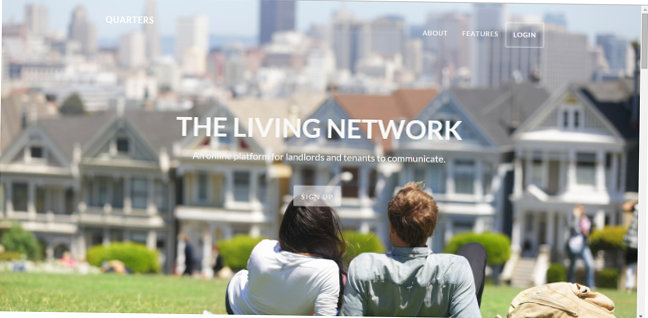
\includegraphics[width=\textwidth]{landing}
\caption{Screen image of Landing page}
\label{fig:landingPage}
\end{figure}

\subsection{Sign Up}
The sign up page is designed to have strong visibility. A new user should be able to know what to do just by looking at the page. The page is simple, straightforward and uncluttered to allow for a quick process. The empty fields afford input. The sign up button is an example of a constraint because it is disabled until the user enters valid input. See Figure \ref{fig:signup}.

\begin{figure}
\centering
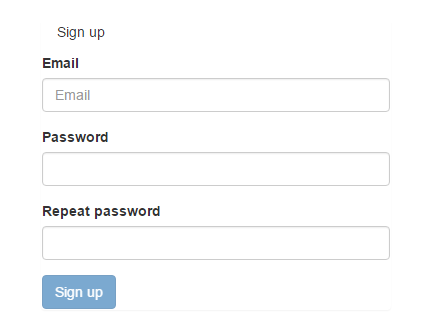
\includegraphics{signup}
\caption{Screen image of Sign Up page}
\label{fig:signup}
\end{figure}

\subsection{Join or Create House}
See \ref{management}.

\subsection{Login}
Designed similarly to the sign up page, the login page has strong visibility. The empty fields afford input. The login button is disabled until the user enters valid input.

\subsection{Navigation bars}
Every page of the application has the same layout for consistency. Each page consists of a top navigation bar and a left navigation bar, and the remaining space is devoted to hold the content of that specific page. The structure of the navigation bars are consistent throughout the application to improve learnability. Fonts, colors and layouts are consistent, as well. The whole user experience, from signing up to logging out, is responsive. This means that regardless of the screen window size, the user will be able to access all functionality of the application. For example, the navigation bars collapse to a toggle menu in smaller screen sizes to ensure the premium screen space is occupied mainly by content with which the user will spend the most time interacting. The intuitive iconography of the navigation bars clearly indicate there are more options hiding deeper down, and thus, demonstrates strong visibility.

\subsection{Bulletin Board}
The bulletin board (bulletin for convenience) is the main page of the application. From here, every other page can be accessed via the navigation bar. Every user's bulletin is personalized based on their activity and their house's activity. Posts take up the majority of the screen space and are listed in chronological order to support the conceptual model. Each post is listed with a corresponding icon that symbolizes the type of activity. A large field is positioned at the top of the bulletin to allow users to share content quickly. When the user clicks on the input field it is highlighted to give feedback to the user that the field is active and input is allowed. See Figure \ref{fig:bulletin}.

\begin{figure}[h]
\centering
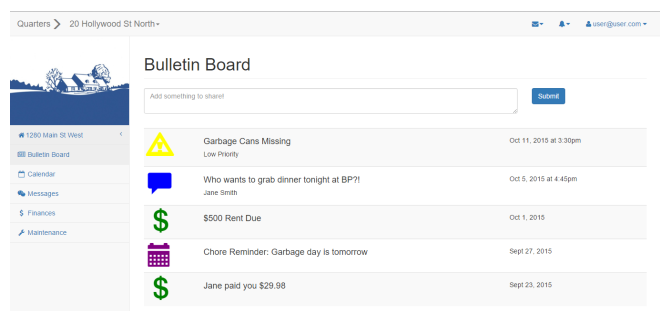
\includegraphics[width=\textwidth]{bulletin}
\caption{Screen image of Bulletin Board page}
\label{fig:bulletin}
\end{figure}

\subsection{House Management}\label{management}
New users are automatically directed to this page after signing up. Returning users can access House Management via the top navigation bar by clicking on the house address. This page is where users can join new houses, create new houses, or add members to a house. This page should be designed with strong feedback including whether the user's actions were successful and what actions they should take next.

\subsection{User Settings}
Users can change their display name on this page. This page is accessible by clicking on the user's email in the top navigation bar.

\subsection{House Settings}
House Settings is accessible via the side navigation bar. Important documents uploaded by members of the house are included here. Documents should be presented following the conceptual model of a stack of "papers", that is, a scaled-down screenshot of each document should be laid out in a grid-like structure.

\subsection{Calendar}
The Calendar resembles the UI of \href{https://apps.google.com/products/calendar/‎}{Google Calendar} because it is a widely used calendar that allows for some familiarity. The checkbox group showcasing different calendars improves visibility of the calendar state. The Calendar should be designed so that users can click on a day or established event to make changes, as opposed to only allowing users to make changes using the buttons positioned above the Calendar. In this way, the natural mapping allows users to interact with the Calendar in an intuitive manner. See Figure \ref{fig:calendar}.

\begin{figure}
\centering
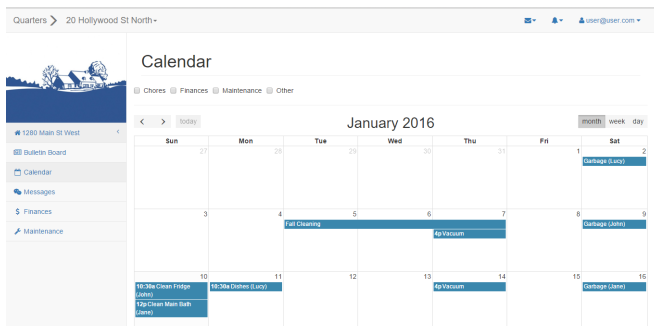
\includegraphics[width=\textwidth]{calendar}
\caption{Screen image of Calendar page}
\label{fig:calendar}
\end{figure}

\subsection{Messages}
A basic chat history of direct messages between two users is displayed here. The messages section is separate from the online users section. An image of the user accompanies each message. Again, a simple, uncluttered interface is important to ensure the user experience is as quick as possible. See Figure \ref{fig:messages}.

\begin{figure}
\centering
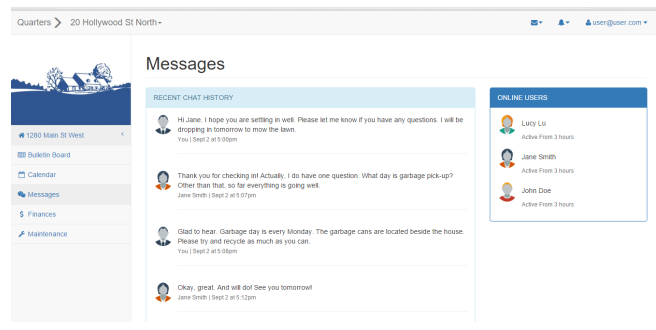
\includegraphics[width=\textwidth]{messages}
\caption{Screen image of Messages page}
\label{fig:messages}
\end{figure}

\subsection{Finances}
The main focus of this page is a table displaying all bills owed and owing. See Figure \ref{fig:finances}.

\begin{figure}
\centering
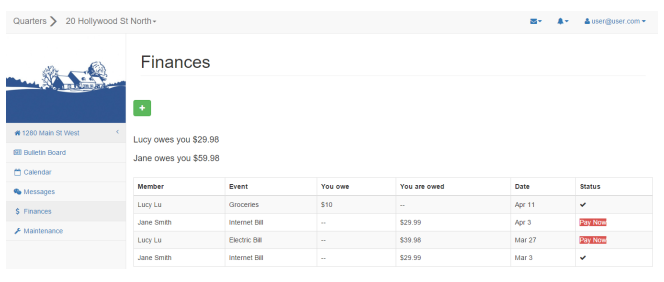
\includegraphics[width=\textwidth]{finances}
\caption{Screen image of Finances page}
\label{fig:finances}
\end{figure}

\subsection{Maintenance}
This section holds a list of maintenance tickets in chronological order. Each ticket is accompanied by a corresponding icon to symbolize the type of ticket. Colors are used to differentiate the priority levels of each ticket. Each ticket is displayed in its own horizontal panel. See Figure \ref{fig:maintenance}.

\begin{figure}
\centering
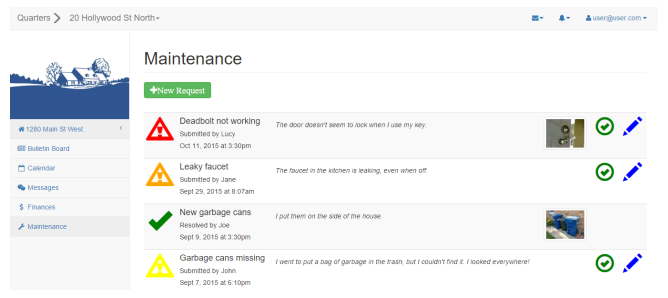
\includegraphics[width=\textwidth]{maintenance}
\caption{Screen image of Maintenance page}
\label{fig:maintenance}
\end{figure}

\subsection{Notifications}
Notifications are accessed via the bell icon displayed in the top navigation bar. Notifications are viewed by clicking on the dropdown menu. Visibility is improved because the navigation bar is displayed on every page, therefore, notifications are displayed on every page. As a result, the user is always aware of application updates. Feedback is improved because the notification icon, the bell, changes color upon a new notification, and then reverts back to its default color to inform the user that they have read the notification.

%Relational database stru


\section{Module Decomposition}

\subsection{Login}
\begin{itemize}
    \item Allows user to login into Quarters application.
\end{itemize}
\subsubsection{Functions}
\begin{itemize}
    \item login(email,pass)
    \begin{itemize}
        \item send login request with user credential to server to be verified.
        \item outputs appropriate error message if credential is incorrect.
        \item redirect user to main application if login is successful.
    \end{itemize}
\end{itemize}

\subsection{Sign Up}
\begin{itemize}
    \item Allows user to register for an account on Quarters.
\end{itemize}
\subsubsection{Functions}
\begin{itemize}
    \item validateEmail(email)
    \begin{itemize}
        \item validate email against database for uniqueness
        \item outputs error if emails is invalid
    \end{itemize}
    \item signup(email,pass)
    \begin{itemize}
        \item send sign up request with user credential to server to be added to database.
        \item redirect user to main application after sign up is successful.
    \end{itemize}
\end{itemize}


\section{Relational Database Structure}
\subsection{ER-Diagram}
See Figure \ref{fig:er}.
\begin{figure}[h]
  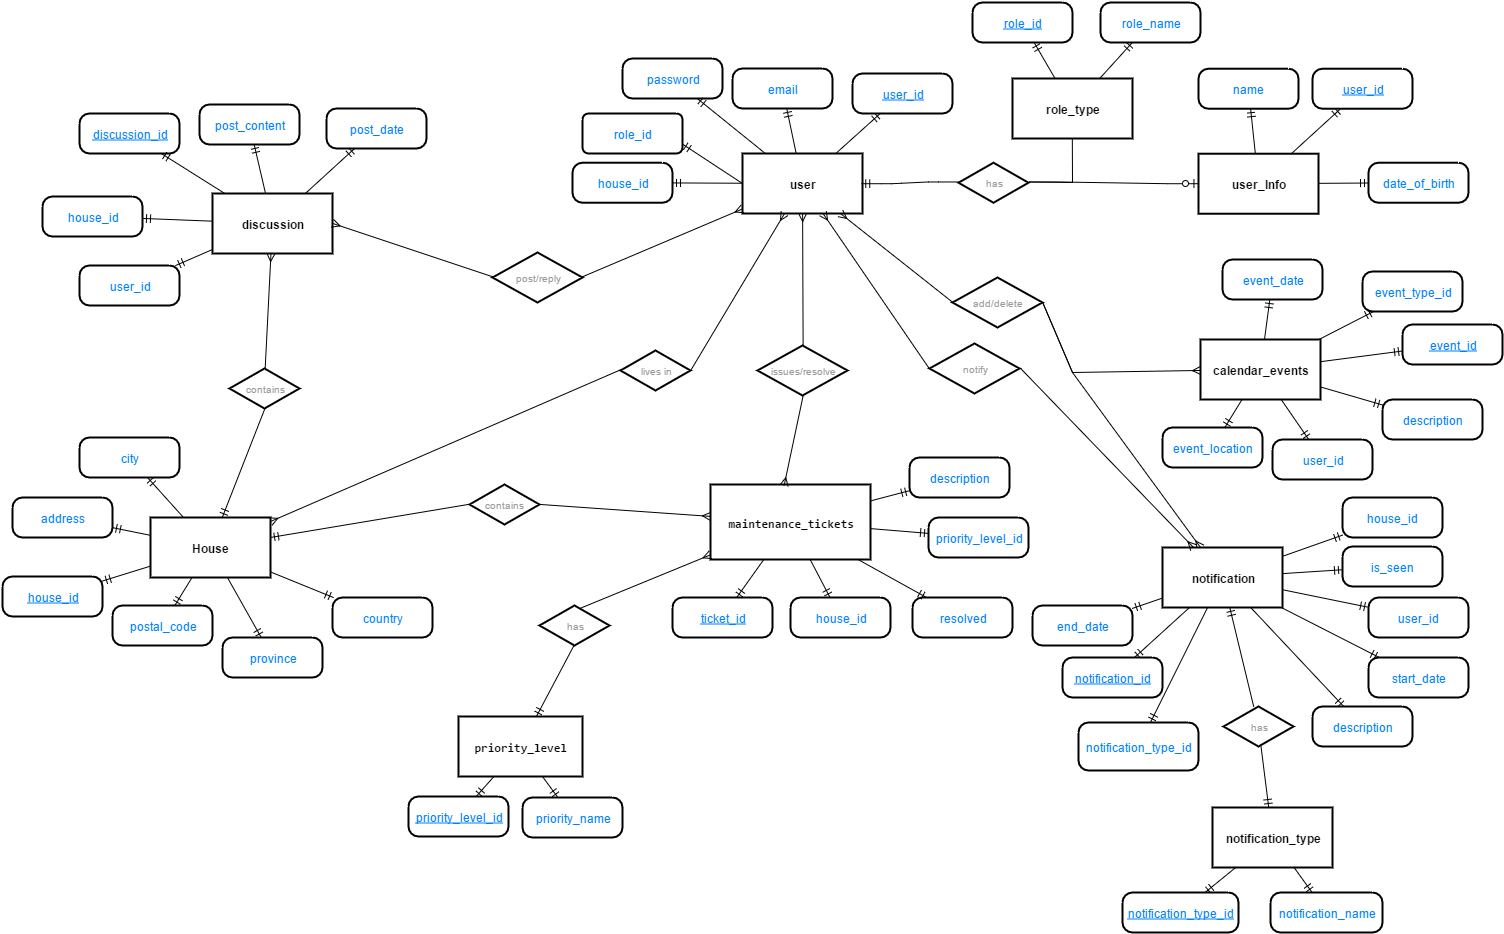
\includegraphics[scale=0.5, keepaspectratio]{images/ER_Diagram.png}
  \caption{ER-Diagram}
  \label{fig:er}
\end{figure}
\subsection{Table Descriptions}
\begin{itemize}
    \item \textbf{user} - Store user credentials(email, password, role type)
    \item \textbf{user\_info} - Store basic user informations(name, birthday etc.)
    \item \textbf{house} - Store house informations (address, postal code, etc.)
    \item \textbf{maintenance\_tickets} - Store maintenance tickets details
    \item \textbf{discussion} - Store discussion posts
    \item \textbf{priority\_level} - Specify priority levels (low, medium, high)
    \item \textbf{role\_type} - Specify role types (tenants, landlord)
    \item \textbf{calendar\_events} - Store calender event details
    \item \textbf{notification} - Store notifications for users
    \item \textbf{notification\_type} - Specify notification types (discussion, events, tickets, joined house, etc.)

\end{itemize}

%
\section{Development Details}
\begin{description}
  \item[Languages of implementation] \hfill
    \begin{itemize}
      \item \href{https://nodejs.org/en/}{NodeJS}
      \item \href{http://www.postgresql.org/}{PostgreSQL}
      \item \href{http://jade-lang.com/}{Jade}
    \end{itemize}
  \item[Supporting frameworks] \hfill
    \begin{itemize}
      \item \href{http://getbootstrap.com/}{Bootstrap}
      \item \href{http://expressjs.com/}{ExpressJS}
    \end{itemize}
  \item[Supporting technology] \hfill
    \begin{itemize}
      \item \href{http://www.ubuntu.com/server}{Ubuntu Server}
    \end{itemize}
\end{description}

%References
\begin{thebibliography}{9}
\bibitem{norman}
Don Norman.
\textit{The Design of Everyday Things -– Revised and Expanded Edition}.
Basic Books, New York, 10-131, 2013.
\end{thebibliography}


\end{document}
